\section{Experimental Results}\label{sec:results}

On EuroSAT the eight runs were almost tied; in Aguascalientes all of them lost most of their
macro-F1, and fine-tuning won back only part of it. We report the results in the order of the
experiments: EuroSAT, Aguascalientes without and with fine-tuning, the input and weight
variants, the cost, the selected model and the Grad-CAM maps. Every configuration was trained
once with seed 0, so we report the highest observed values and make no claim that one model is
better than another.

\subsection{EuroSAT}

All eight runs reached almost the same score on the EuroSAT test set. Table~\ref{tab:eurosat}
shows that macro-F1 ranged from \EuroSATMin{} to \EuroSATMax, and accuracy followed the same
pattern. ResNet-50/MS13/SSL4EO had the highest observed value in both columns. This means that
EuroSAT alone does not separate the models.

\begin{table}[t]
\centering
\footnotesize
\caption{EuroSAT test set (10 classes): overall accuracy and macro-F1 of the eight runs. Best value per column in bold.}
\label{tab:eurosat}
\begin{tabular}{lrr}
\toprule
Run & Accuracy & Macro-F1 \\
\midrule
ResNet-50 / RGB / ImageNet & 0.984 & 0.983 \\
ResNet-50 / MS13 / ImageNet & 0.985 & 0.985 \\
ResNet-50 / MS13 / SSL4EO & \textbf{0.993} & \textbf{0.993} \\
EfficientNet-B0 / RGB / ImageNet & 0.984 & 0.984 \\
EfficientNet-B0 / MS13 / ImageNet & 0.985 & 0.985 \\
ViT-S / RGB / ImageNet & 0.991 & 0.991 \\
ViT-S / MS13 / ImageNet & 0.990 & 0.990 \\
ViT-S / MS13 / SSL4EO & 0.987 & 0.987 \\
\bottomrule
\end{tabular}
\end{table}


The training curves tell the same story. Fig.~\ref{fig:convergence} shows the validation
macro-F1 per epoch: every run reached a high value within the first few epochs and changed
little afterwards. The curves differ mainly in the first epoch, where the two ResNet-50 runs
with ImageNet weights started lowest. With 13 bands, the SSL4EO-S12 run of each model started
higher than the ImageNet run of the same model, although ViT-S/RGB/ImageNet started slightly
above ViT-S/MS13/SSL4EO. The epochs needed to reach 95\,\% of the best validation macro-F1 did
not separate the models either: every run needed at most \EpochsToNinetyFiveMax{} epochs.

\begin{figure}[t]
\centering
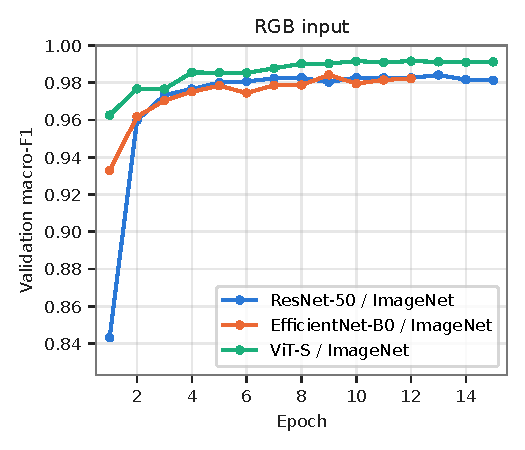
\includegraphics[width=\columnwidth]{convergence_rgb}\\[2pt]
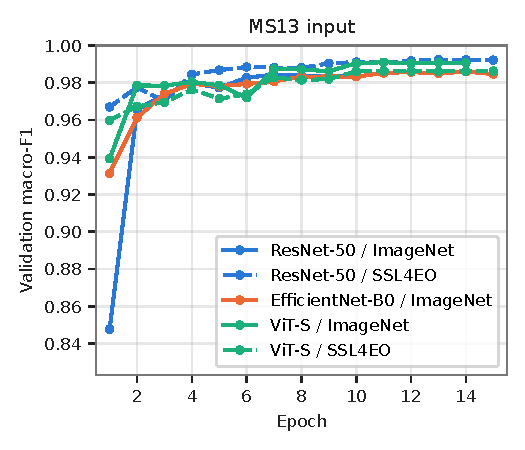
\includegraphics[width=\columnwidth]{convergence_ms13}
\caption{Validation macro-F1 on EuroSAT per training epoch. Top: RGB input. Bottom: 13-band
(MS13) input; dashed lines are the SSL4EO-S12 runs.}
\label{fig:convergence}
\end{figure}

\subsection{Aguascalientes without fine-tuning}

The models lost most of their EuroSAT performance when we tested them on Aguascalientes
without local training. The zero-shot column of Table~\ref{tab:ags} shows macro-F1 between
\ZeroShotMin{} and \ZeroShotMax{} over the nine classes. The drop, the EuroSAT F1 minus the
zero-shot F1, ranged from \DropMin{} to \DropMax. In other words, most of what the models
learned in Europe did not carry over to semi-arid Aguascalientes.

\begin{table*}[t]
\centering
\footnotesize
\caption{Macro-F1 on the Aguascalientes test split. The class set is the 9 classes with at least 10 test patches (1 class excluded and reported separately). EuroSAT F1 is the macro-F1 of the EuroSAT test result over the same classes. Drop = EuroSAT F1 minus zero-shot; recovery = (fine-tuned minus zero-shot) / drop, shown as -- when the drop is not positive. Best F1 per column in bold.}
\label{tab:ags}
\begin{tabular}{lrrrrrrr}
\toprule
Run & EuroSAT F1 & Zero-shot & Head & Last block & Drop & Rec. head & Rec. last block \\
\midrule
ResNet-50 / RGB / ImageNet & 0.983 & 0.259 & 0.308 & 0.278 & 0.724 & 0.068 & 0.026 \\
ResNet-50 / MS13 / ImageNet & 0.984 & 0.271 & 0.339 & 0.371 & 0.713 & 0.095 & 0.140 \\
ResNet-50 / MS13 / SSL4EO & \textbf{0.993} & \textbf{0.354} & 0.372 & \textbf{0.525} & 0.639 & 0.029 & 0.268 \\
EfficientNet-B0 / RGB / ImageNet & 0.984 & 0.271 & 0.275 & 0.400 & 0.713 & 0.006 & 0.181 \\
EfficientNet-B0 / MS13 / ImageNet & 0.984 & 0.196 & 0.217 & 0.361 & 0.788 & 0.027 & 0.209 \\
ViT-S / RGB / ImageNet & 0.991 & 0.326 & \textbf{0.380} & 0.441 & 0.665 & 0.081 & 0.173 \\
ViT-S / MS13 / ImageNet & 0.989 & 0.287 & 0.340 & 0.361 & 0.703 & 0.076 & 0.106 \\
ViT-S / MS13 / SSL4EO & 0.987 & 0.287 & 0.305 & 0.428 & 0.699 & 0.025 & 0.201 \\
\bottomrule
\end{tabular}
\end{table*}


Fig.~\ref{fig:ags_f1}(a) shows where the loss happened. HerbaceousVegetation had the highest
per-class F1 in every run, while Forest and Pasture were at or near zero in every run. River
appears hatched because it has only seven test patches and is reported separately. The pattern
is the same for the three architectures, both inputs and both kinds of weights.

\begin{figure*}[t]
\centering
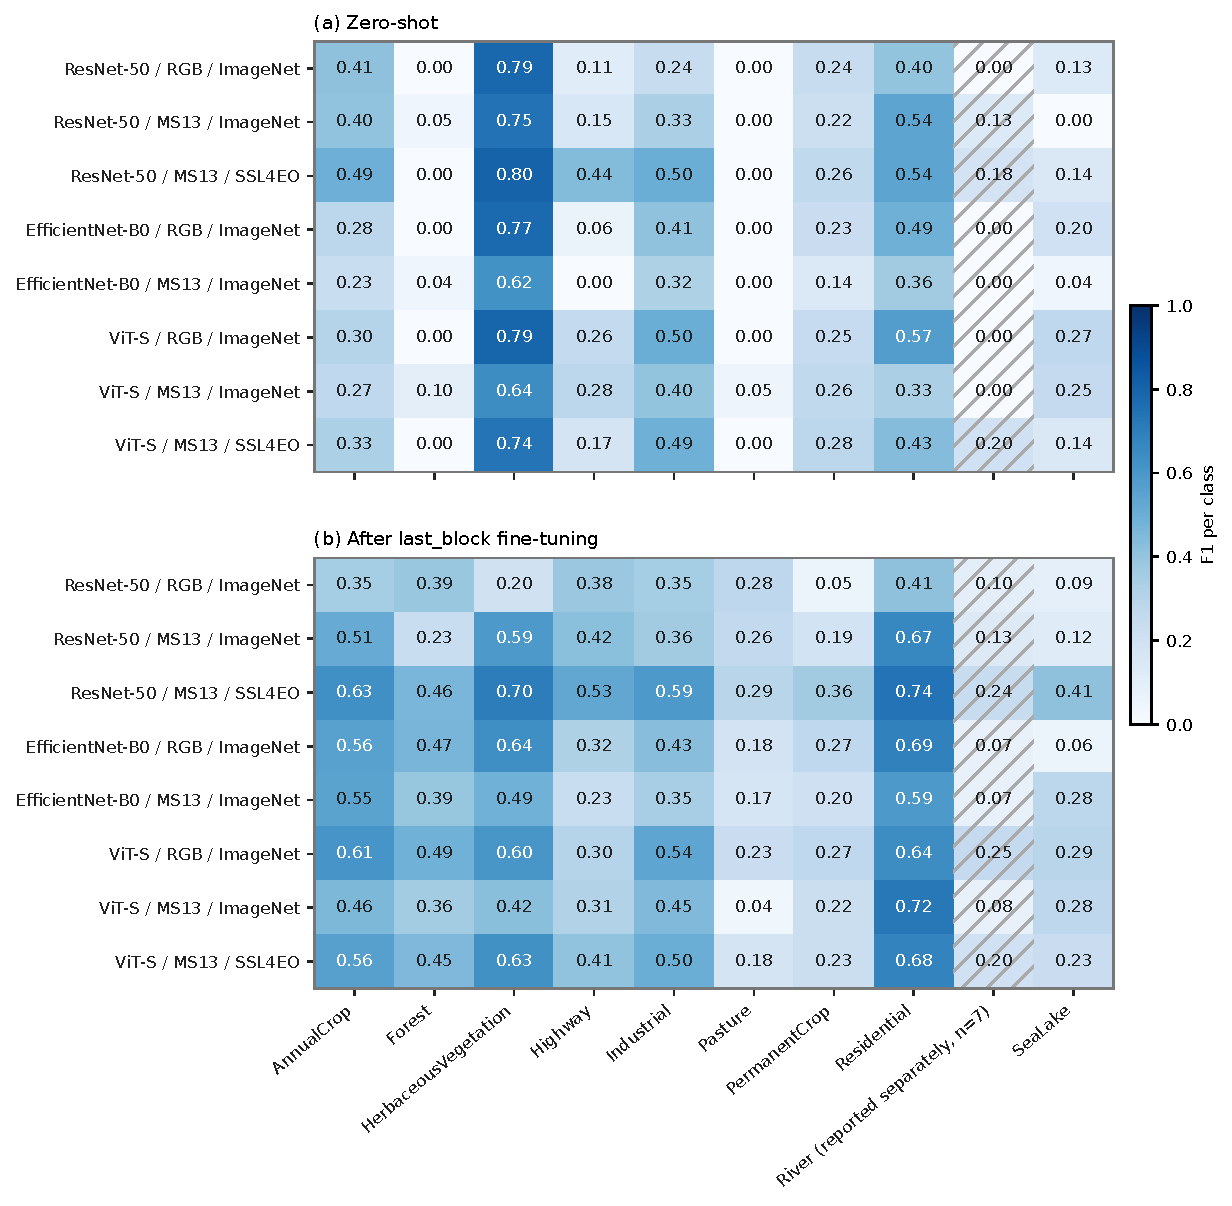
\includegraphics[width=0.75\textwidth]{ags_f1_per_class}
\caption{Per-class F1 on the Aguascalientes test split for the eight runs. (a) Zero-shot.
(b) After \texttt{last\_block} fine-tuning. River (hatched) has too few test patches and is
reported separately.}
\label{fig:ags_f1}
\end{figure*}

The confusion matrix shows the same collapse from the side of the predictions.
Fig.~\ref{fig:confusion}(a) gives the zero-shot confusion matrix of the model we selected later
(Section~\ref{sec:selected}). Most errors fell in the HerbaceousVegetation and PermanentCrop
columns; for example, every Forest test patch was predicted as HerbaceousVegetation. This means
that, without local training, the predictions concentrated in two classes, one of them the
largest class of the test set.

\begin{figure*}[t]
\centering
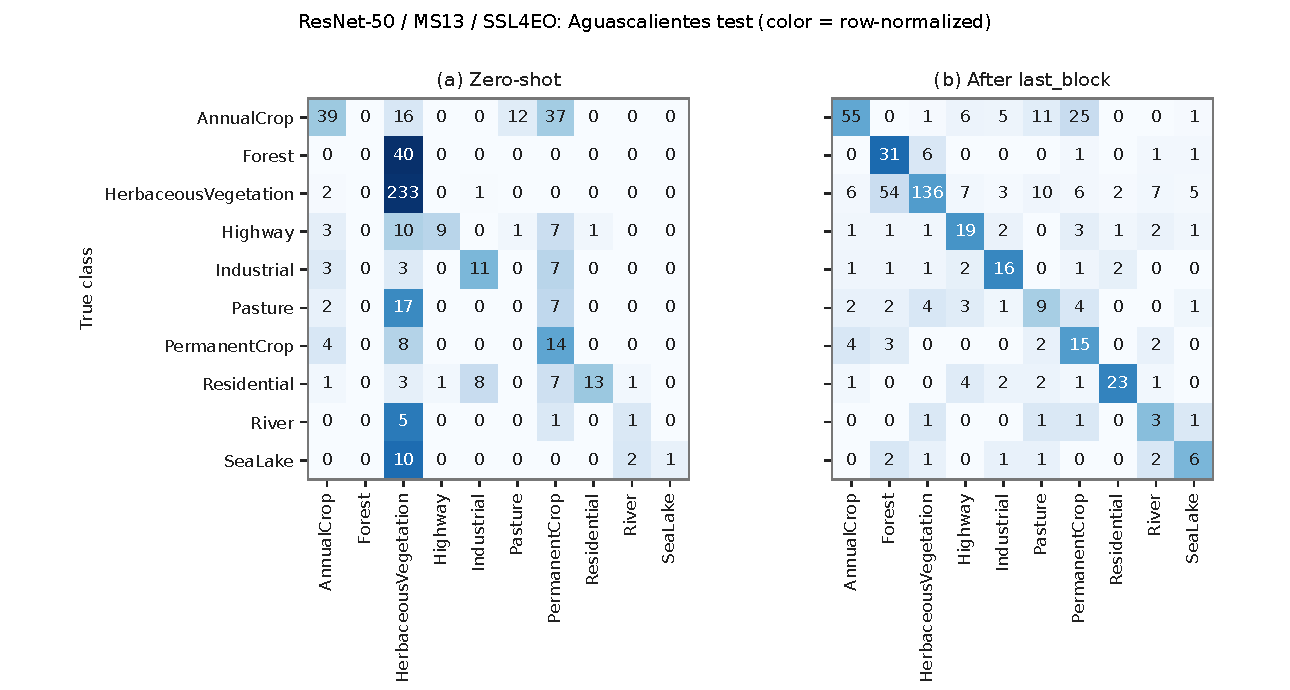
\includegraphics[width=\textwidth]{confusion_selected}
\caption{Confusion matrices of the selected model, ResNet-50/MS13/SSL4EO, on the
Aguascalientes test split. (a) Zero-shot. (b) After \texttt{last\_block} fine-tuning. Cells
show patch counts; the color is normalized per row (true class).}
\label{fig:confusion}
\end{figure*}

\subsection{Fine-tuning on Aguascalientes}

Fine-tuning won back only part of the drop, and how much depended on the mode. The Head and
Last block columns of Table~\ref{tab:ags} give the macro-F1 after each mode, and
Fig.~\ref{fig:drop_recovery} shows the drop (a) and the recovery (b) of every run. With
\texttt{head}, the recovery was at most \HeadRecoveryMax, so training only the classifier
barely changed the scores. With \texttt{last\_block}, the recovery ranged from \RecoveryMin{}
to \RecoveryMax. This means that the largest part of the drop remained after fine-tuning in
every run.

\begin{figure*}[t]
\centering
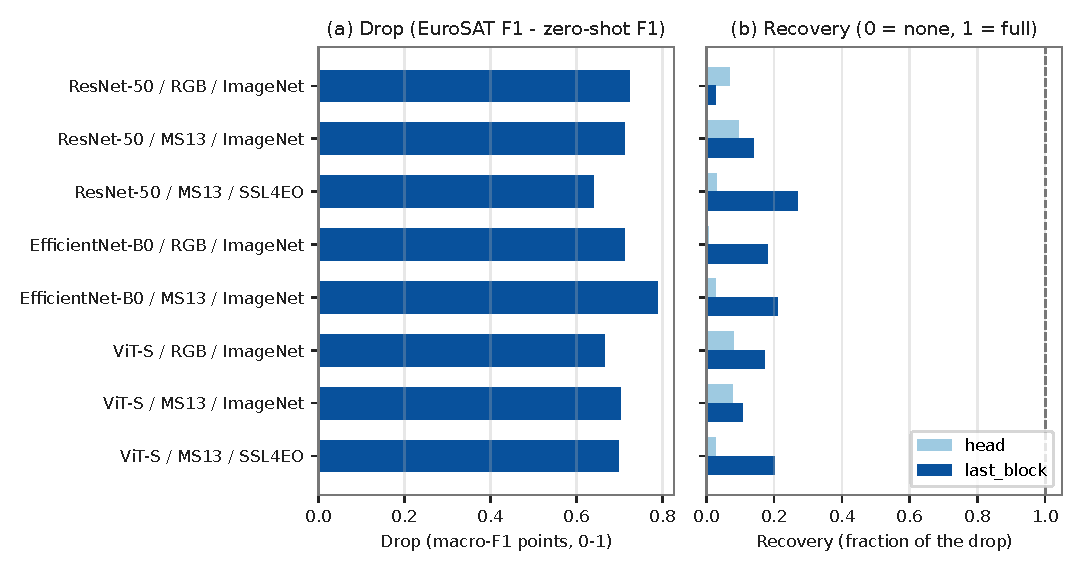
\includegraphics[width=\textwidth]{drop_recovery}
\caption{(a) Drop from EuroSAT macro-F1 to Aguascalientes zero-shot macro-F1 for each run.
(b) Recovery after \texttt{head} and \texttt{last\_block} fine-tuning, as a fraction of the
drop; the dashed line marks full recovery.}
\label{fig:drop_recovery}
\end{figure*}

One run did not follow the general order of the two modes. In every run except
ResNet-50/RGB/ImageNet, \texttt{last\_block} gave a higher macro-F1 than \texttt{head}. For
ResNet-50/RGB/ImageNet, macro-F1 after \texttt{last\_block} (\ResNetRgbLastBlock) was below
that after \texttt{head} (\ResNetRgbHead). Its Aguascalientes accuracy also fell, from
\ResNetRgbZeroShotAcc{} zero-shot to \ResNetRgbLastBlockAcc{} after \texttt{last\_block}.

The fall in accuracy was not limited to that run. In \AccuracyDropRuns{} of the \NumRuns{}
runs, \texttt{last\_block} lowered the Aguascalientes accuracy below its zero-shot value while
it raised macro-F1. This trade-off is consistent with the class-weighted loss of
Eq.~\eqref{eq:class_weights}, which shifts predictions away from the dominant
HerbaceousVegetation class. Fig.~\ref{fig:ags_f1}(b) shows both sides of it: Forest and Pasture
are no longer at zero in any run, and HerbaceousVegetation F1 is lower than zero-shot in every
run.

\subsection{Input bands and pre-trained weights}

Whether 13 bands helped depended on the model. Comparing the RGB and 13-band runs with ImageNet
weights in Table~\ref{tab:ags}, only ResNet-50 scored higher with 13 bands, both zero-shot and
after \texttt{last\_block}. EfficientNet-B0 and ViT-S scored lower with 13 bands in both
columns. In other words, our results do not support a general rule that more bands help under
this domain shift.

With 13 bands, the SSL4EO-S12 runs reached a higher macro-F1 after \texttt{last\_block} than
the ImageNet runs, for both ResNet-50 and ViT-S. Zero-shot, ResNet-50 was also higher with
SSL4EO-S12, while ViT-S gave the same value at three decimals with both kinds of weights. On
EuroSAT, ViT-S/MS13/SSL4EO was slightly lower than its ImageNet counterpart
(Table~\ref{tab:eurosat}). Because the SSL4EO-S12 runs also used a different normalization,
$x/\num{10000}$, these gaps cannot be credited to the weights alone. In the same way,
\texttt{last\_block} trains a different share of the parameters of each architecture, so we
leave the CNN versus ViT comparison after fine-tuning to Section~\ref{sec:discussion}.

\subsection{Computational cost}

Table~\ref{tab:cost} lists the cost of the eight EuroSAT runs. Peak memory is the memory
reserved by the MPS driver, not the memory that the weights and activations of the model need
on their own. ViT-S reserved the most: at least \PeakMemVitMin~GiB, against at most
\PeakMemCnnMax~GiB for the CNNs. Inference throughput ranged from \PatchesPerSecMin{} to
\PatchesPerSecMax{} patches/s, and each 13-band run had a lower throughput than the RGB run of
the same model.

\begin{table*}[t]
\centering
\footnotesize
\caption{Training cost of the eight EuroSAT runs on an Apple M2 Pro (fp32). Peak memory is the memory reserved by the MPS driver. Patches/s is inference throughput on the EuroSAT test set.}
\label{tab:cost}
\begin{tabular}{lrrrrr}
\toprule
Run & Params (M) & Train time (min) & Time/epoch (s) & Peak mem. (GiB) & Patches/s \\
\midrule
ResNet-50 / RGB / ImageNet & 23.5 & 58.3 & 233 & 4.31 & 208 \\
ResNet-50 / MS13 / ImageNet & 23.6 & 42.0 & 252 & 4.31 & 184 \\
ResNet-50 / MS13 / SSL4EO & 23.6 & 62.9 & 252 & 4.31 & 183 \\
EfficientNet-B0 / RGB / ImageNet & 4.0 & 45.5 & 227 & 4.33 & 233 \\
EfficientNet-B0 / MS13 / ImageNet & 4.0 & 57.8 & 231 & 4.33 & 214 \\
ViT-S / RGB / ImageNet & 21.7 & 54.6 & 218 & 5.18 & 236 \\
ViT-S / MS13 / ImageNet & 22.7 & 55.3 & 237 & 5.25 & 199 \\
ViT-S / MS13 / SSL4EO & 22.7 & 59.3 & 237 & 5.25 & 199 \\
\bottomrule
\end{tabular}
\end{table*}


Total training time is a weak basis for comparison, because early stopping ended the runs at
different epochs (Fig.~\ref{fig:convergence}). Time per epoch is the comparable column, and it
was similar across the three models. EfficientNet-B0 has far fewer parameters than ResNet-50 and
ViT-S, yet its time per epoch was close to theirs. This means that, on our hardware, the number
of parameters did not predict the training time.

\subsection{Selected model}\label{sec:selected}

Applying the selection rule fixed in Section~\ref{sec:methodology}, we selected
ResNet-50/MS13/SSL4EO with \texttt{last\_block} fine-tuning. Its Aguascalientes macro-F1 was
\AgsLastBlockBest, \SelectionMargin{} above the runner-up, which is wider than the tie-break
margin, so the throughput rule was not needed. Since only ResNet-50 and ViT-S have SSL4EO-S12
runs, we also applied the rule to the six ImageNet runs as a secondary result, where the three
models compete on equal weights. There, ViT-S/RGB/ImageNet came first with
\ImageNetLastBlockBest, \ImageNetSelectionMargin{} above the next run, again without a
tie-break.

Fig.~\ref{fig:confusion}(b) shows the selected model after \texttt{last\_block}. Compared with
panel (a), the predictions now spread along the diagonal instead of piling up in the
HerbaceousVegetation column. The largest off-diagonal cell is HerbaceousVegetation predicted as
Forest. In other words, the main error changed direction: from most patches being called
HerbaceousVegetation to part of HerbaceousVegetation being called Forest.

\subsection{Grad-CAM}

Fig.~\ref{fig:gradcam} shows the Grad-CAM maps of the RGB ImageNet run of each model, without
fine-tuning, on EuroSAT (a) and Aguascalientes (b). We drew one test patch per class at random
with seed 0, for six classes, so the patches were not chosen to make a point; the list and the
rule are stored with the figures. Under each map is the predicted class, marked as correct or
wrong. On EuroSAT all predictions but one are correct, while on Aguascalientes most are wrong,
and most of the wrong ones are HerbaceousVegetation.

\begin{figure*}[t]
\centering
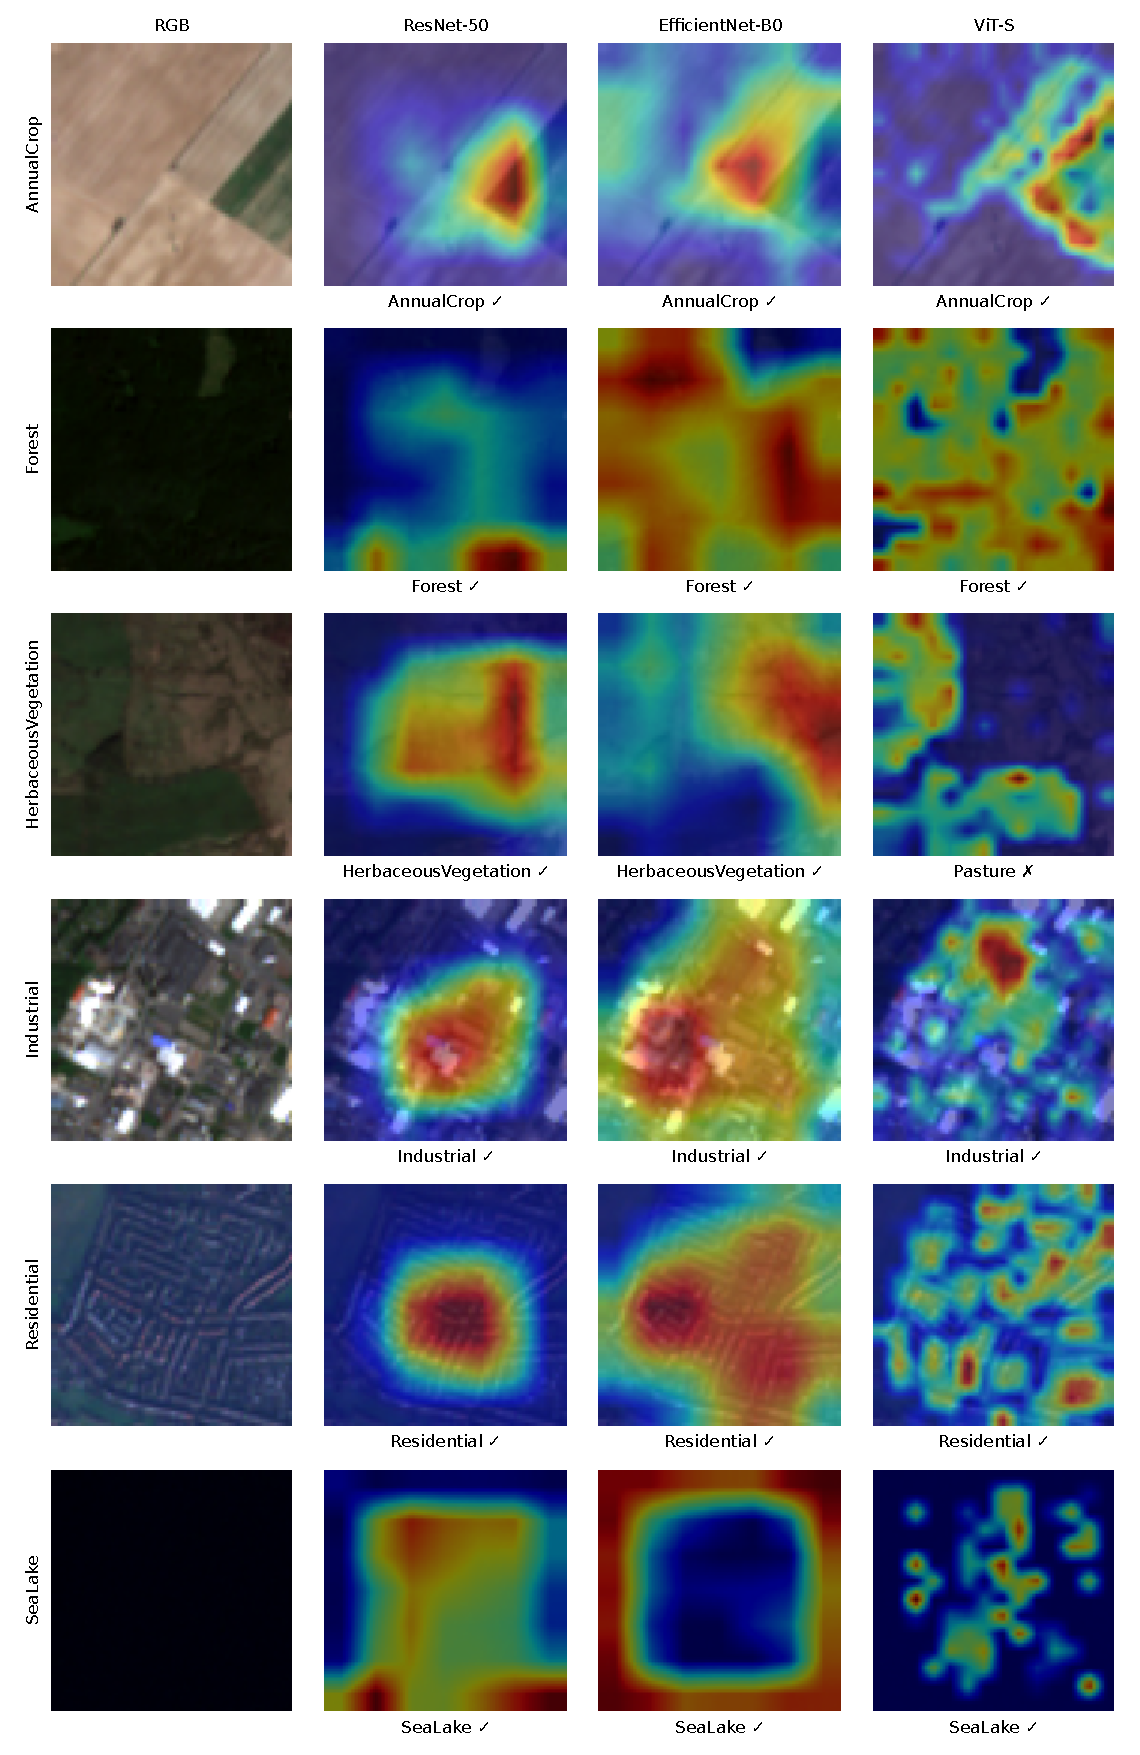
\includegraphics[width=0.48\textwidth]{gradcam_eurosat}\hfill
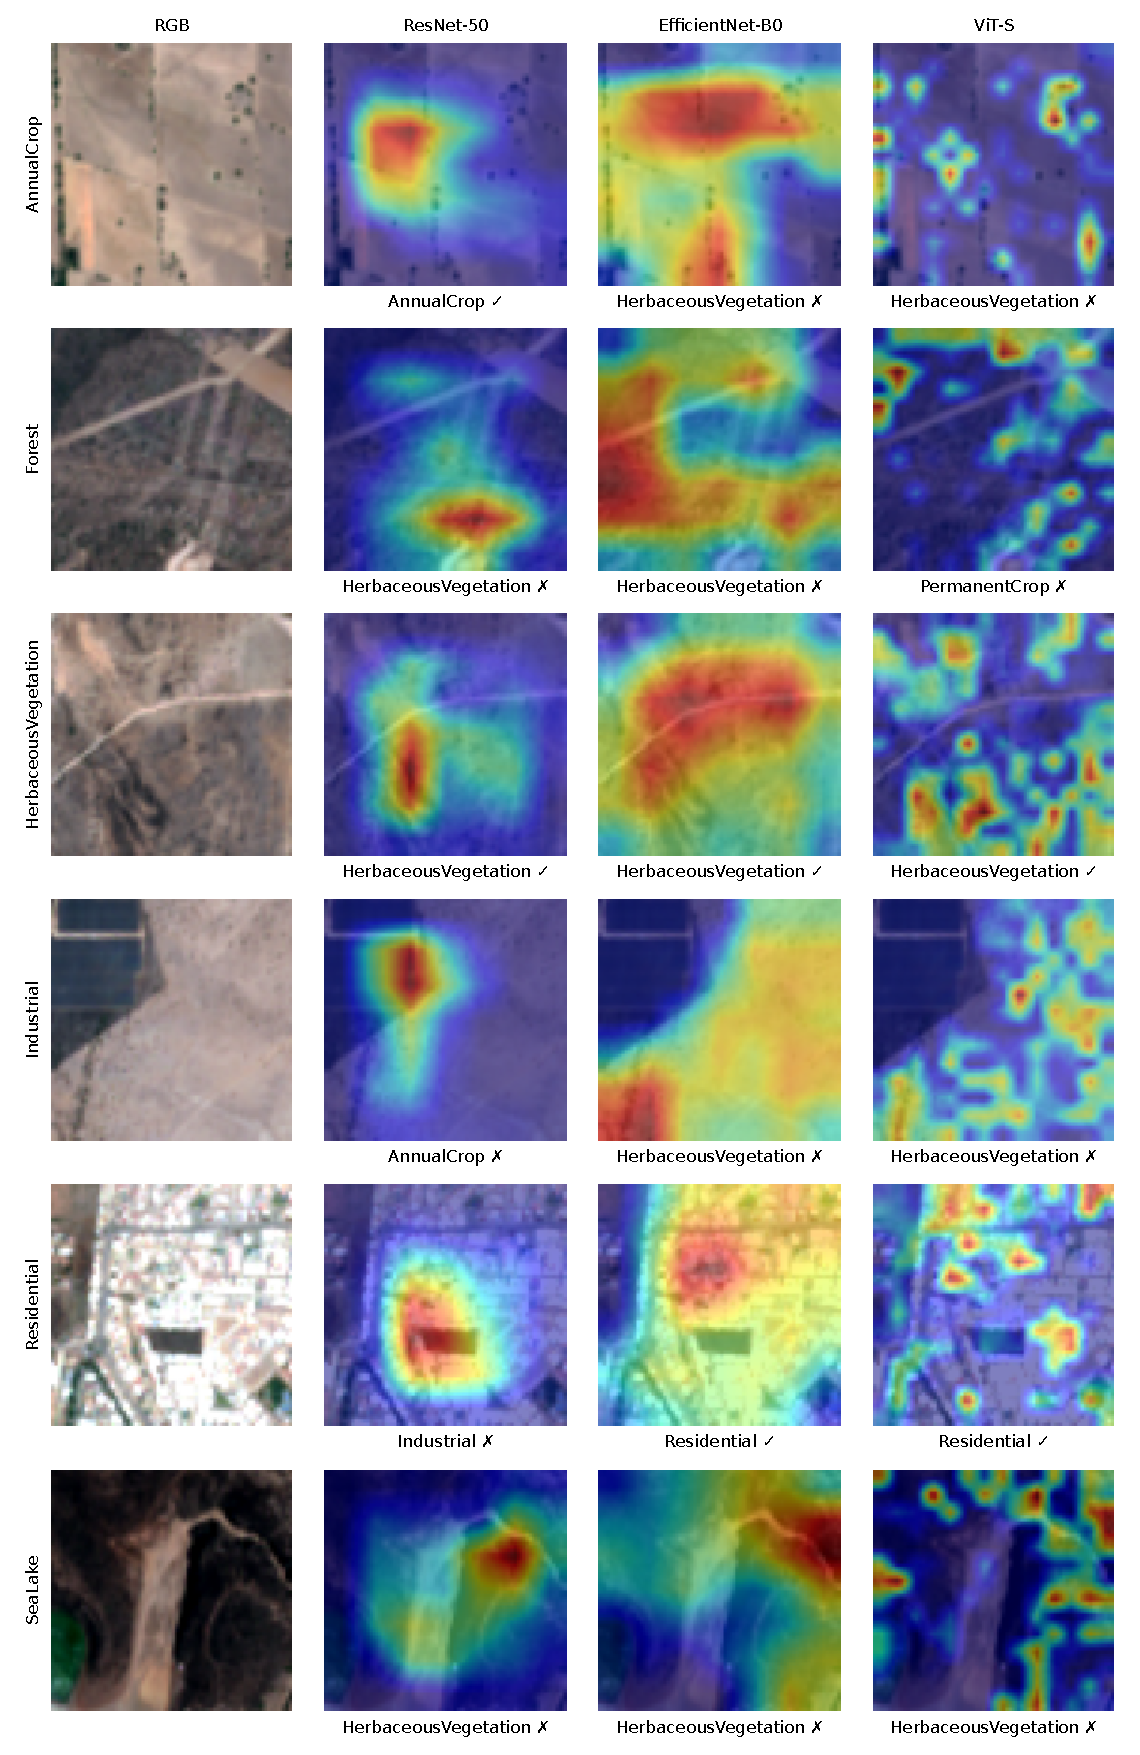
\includegraphics[width=0.48\textwidth]{gradcam_ags}
\caption{Grad-CAM maps of the RGB ImageNet runs, without fine-tuning, on one random test patch
per class (seed 0). (a) Left: EuroSAT. (b) Right: Aguascalientes. Columns: RGB patch,
ResNet-50, EfficientNet-B0 and ViT-S. Under each map: the predicted class, with a check mark if
correct and a cross if wrong.}
\label{fig:gradcam}
\end{figure*}

The two families of models produce maps of a different shape. CNN maps are smooth and
concentrated on one compact region of the patch, sometimes two. ViT-S maps are made of many
small spots spread over the whole patch. In Aguascalientes, many maps fall away from the object
that defines the class. The Industrial cell of Fig.~\ref{fig:gradcam}(b) is a solar park,
seen as a dark rectangle of panels at the top left. The maximum of the ResNet-50 map lies on
the edge of the panels. The maximum of EfficientNet-B0 falls in the lower-left corner, and the
spots of ViT-S spread over the bare ground. None of the three models predicted Industrial for
this patch.

Fig.~\ref{fig:gradcam_selected} compares the selected model before and after
\texttt{last\_block} on the Aguascalientes patches of Fig.~\ref{fig:gradcam}(b). The
HerbaceousVegetation and SeaLake rows are replaced by two HerbaceousVegetation patches drawn at
random with seed 0 among those that the fine-tuned model predicts as Forest; that is, they were
chosen to show the main error of Fig.~\ref{fig:confusion}(b). Both were correct zero-shot and
became Forest after \texttt{last\_block}. The AnnualCrop patch changed from a wrong prediction
to a correct one, the Forest and Industrial patches stayed wrong, and the Residential maps are
almost the same before and after. We leave the interpretation of all these maps to
Section~\ref{sec:discussion}.

\begin{figure*}[t]
\centering
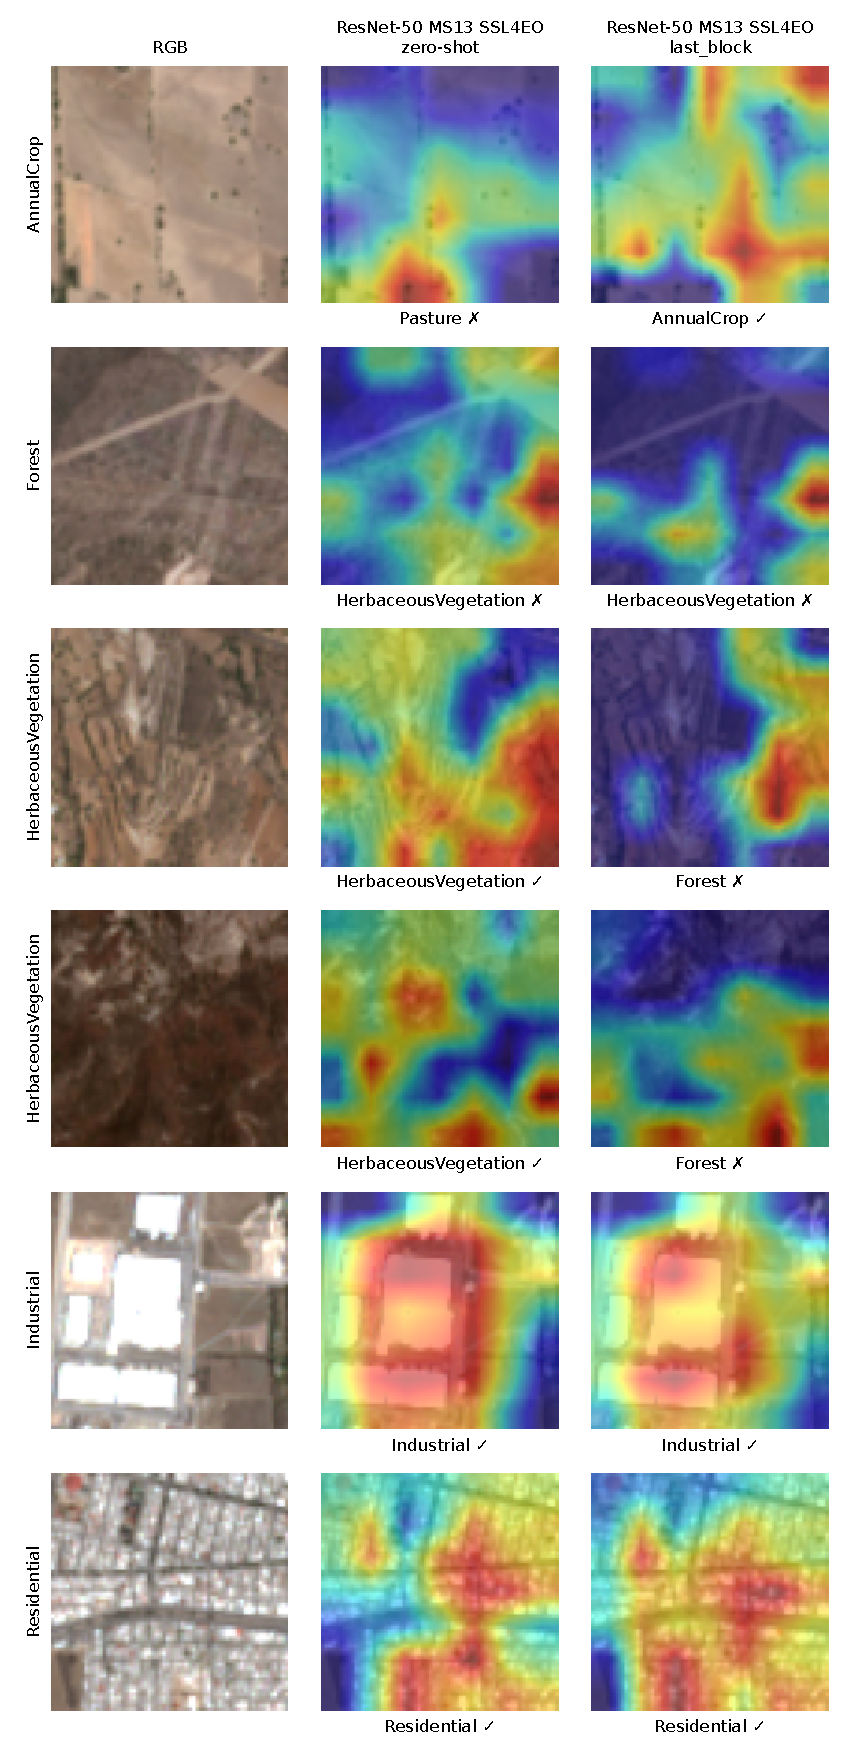
\includegraphics[height=0.5\textheight]{gradcam_selected}
\caption{Grad-CAM maps of the selected model, ResNet-50/MS13/SSL4EO, on Aguascalientes test
patches. Columns: RGB patch, zero-shot and after \texttt{last\_block}. The two
HerbaceousVegetation rows are random patches (seed 0) among those predicted as Forest after
\texttt{last\_block}; the other rows are the patches of Fig.~\ref{fig:gradcam}(b).}
\label{fig:gradcam_selected}
\end{figure*}
